\documentclass[10pt,a4paper]{report}

\usepackage[utf8]{inputenc}
\usepackage[french]{babel}
\usepackage[T1]{fontenc}
\usepackage{amsmath}
\usepackage{amsfonts}
\usepackage{amssymb}
\usepackage{graphicx}
\usepackage{lmodern}
\usepackage{hyperref}
\usepackage{url}
\usepackage{xspace}
\usepackage{tikz}
\usepackage{listings}
\usepackage{caption}
\usepackage{subcaption}
\usepackage{enumitem}
%\usepackage{feynmp}
%\usepackage{tikz-feynman}

\usepackage[left=2cm,right=2cm,top=2cm,bottom=2cm]{geometry}

%%%%%%%%%%%%%%%%%%%%%%%%%%%%% Page de garde %%%%%%%%%%%%%%%%%%%%%%%%%%%%%
\author{Alexia \textsc{HOCINE}}

\title{
	Détecteur SDHCAL pour le signal  $ e^{+} e^{-} \longrightarrow \nu \nu h $ :\\
	Optimisation et Adaptation de l'analyse de données\\pour le Projet FCC 
}
%Stage M2 Physique, parcours SUBA\\Université de Claude Bernard Lyon 1
\date{Juillet 2022}

%%%%%%%%%%%%%%%%%%%%%%%%%%%%% Raccourçi %%%%%%%%%%%%%%%%%%%%%%%%%%%%%

% raccourci français
\newcommand{\cad}{c'est-à-dire\xspace}
\newcommand{\qqs}{quelque soit\xspace}
\newcommand{\MS}{Modèle Standard\xspace}


% nom informatique
\newcommand{\ROOT}{\texttt{ROOT}\xspace}
\newcommand{\SLCIO}{\texttt{SLCIO}\xspace}
\newcommand{\iLCSoft}{\texttt{iLCSoft}\xspace}
\newcommand{\LCIO}{\texttt{LCIO}\xspace}
\newcommand{\Marlin}{\texttt{Marlin}\xspace}
\newcommand{\Gaudi}{\texttt{Gaudi}\xspace}
\newcommand{\FCC}{\texttt{FCC}\xspace}
\newcommand{\EDMhep}{\texttt{EDM4hep}\xspace}

\newcommand{\nnhAnalysis}{\texttt{nnhAnalysis}\xspace}

\newcommand{\original}{\texttt{original}\xspace}
\newcommand{\ilcsoft}{\texttt{ilcsoft}\xspace}
\newcommand{\fcc}{\texttt{fcc}\xspace}

\newcommand{\minidstmarker}{\texttt{miniDSTMaker}\xspace}
\newcommand{\convert}{\texttt{convert}\xspace}
\newcommand{\processor}{\texttt{processor}\xspace}
\newcommand{\analysis}{\texttt{analysis}\xspace}


% nom de particules
\newcommand{\particle}[1]{$\texttt{#1}$}

\newcommand{\bbar}{\overline{b}}
\newcommand{\Wstar}{W^{\star}}

\newcommand{\electron}{e^{+}}
\newcommand{\positron}{e^{-}}

\newcommand{\nnh}{\nu \nu h}

% processus courants
\newcommand{\bb}{$\mathrm{b\bbar}$\xspace}
\newcommand{\WW}{$\mathrm{W\Wstar}$\xspace}

% physique
\newcommand{\GeV}{\mathrm{GeV}\xspace}
\newcommand{\TeV}{\mathrm{TeV}\xspace}
\newcommand{\MeV}{\mathrm{MeV}\xspace}

\newcommand{\m}[1]{m_\mathrm{#1}}
\newcommand{\mH}{m_\mathrm{H}}
\newcommand{\mW}{m_\mathrm{W}}

\newcommand{\vmH}{125,25}
\newcommand{\vmW}{80,377}
\newcommand{\vs}{250}
\newcommand{\vGF}{1,166\,378\,8 \times 10^{-5}}
\newcommand{\vhc}{0,389\,379\,365\,648} % (hbar c)^2


\newcommand{\GF}{G_\mathrm{F}}
\newcommand{\gHWW}{g_\mathrm{HWW}}

% LaTeX

\newcommand{\doToList}[1]{{\color{red}#1}}
\newcommand{\Figure}[1]{[\textsc{Figure~#1}]}


%%%%%%%%%%%%%%%%%%%%%%%%%%%%% corps du document %%%%%%%%%%%%%%%%%%%%%%%%%%%%%

\begin{document}

% Page de Garde

\begin{titlepage}
	\begin{center}
		
    		\vspace*{3cm}

    		\LARGE
    		\textbf{Détecteur SDHCAL pour le signal  $ e^{+} e^{-} \longrightarrow \nu \nu h $ :\\Optimisation et Adaptation de l'analyse de données\\pour le Projet FCC}

    		\vspace{1.5cm}

    		Alexia \textsc{HOCINE}\\
    		\vspace{0.4cm}
    		\large 
    			Étudiante en M2 Physique SUBA à l'UCBL1
    		
		\vspace{1.5cm}
		\Large
		Supervisé par Gérald \textsc{Grenier}\\
    		\vspace{0.4cm}
    		\large 
    			Maître de Conférence - UCBL1\\
    			Enseignant-Chercheur - IP2I, CNRS, IN2P3\\
    			Membre des collaborations CALICE, CMS et ILD\\
    			Corresponsable du groupe SDHCAL au sein de la collaboration CALICE

    		\vfill

		
\includegraphics[width=5cm]{../img/Logo_IP2I.png}
 		
\includegraphics[width=5cm]{../img/UdL-logo.png}

		\vspace{3cm} 

    		Rapport de Stage - Master 2 Physique SUBA\\
    		Université de Claude Bernard Lyon 1 \\    		

    		\vspace{1.5cm}
    		
    		Avril-Juillet 2022
    
 		
	\end{center}

\end{titlepage}

\tableofcontents

ev Introduction

\chapter{Introduction}

\section{La Physique des Collisionneurs}

Le principe des collisionneurs est simple, on accélère des particules à des 
énergies cinétiques suffisantes pour provoquer des collisions inélastiques, et ainsi comprendre les interactions fondamentales et les constituants élémentaires de la matière.\\

On distingue 2 familles de collisionneurs en fonction des particules qui sont utilisés.

\subsection{Collisionneurs hadroniques}

Les collisionneurs hadroniques utilisent des hadrons, qui sont des 
particules complexes composées de 3 quarks et de gluons\footnote{Gluon : boson médiateur de l'interaction forte qui maintiennent les quarks ensembles.}. 
Par exemple au LHC\footnote{LHC : Large Hadron Collider, CERN}, on utilise des protons, composés de 2 quarks up et d'1 quark down. 

Comme il s'agit de particules composites, ce sont pas les protons qui collisionnent directement mais ces constituants, appelés partons. 
Chacun porte une fraction indéterminée de l'énergie du proton. 
On ignore donc l'énergie de la collision en amont, il s'agit d'un paramètre libre. 

C'est pourquoi, ils sont utiles pour la découverte de nouvelles particules de masse inconnue, puisqu'ils permettent de balayer tout le spectre de masse sous la gamme d'énergie du collisionneur (au LHC < 14 $\TeV$)\footnote{D'où l'intérêt de nouveaux collisionneurs à des énergies plus élevées et donc des masses de particules produites plus lourdes.}.

\subsection{Collisionneurs leptoniques}

En revanche, les collisionneurs leptoniques utilisent des leptons, qui sont des particules élémentaires. 
Comme le LEP\footnote{LEP : Large Electron-Positron, le prédécesseur du LHC, même tunnel}, qui collisionnait des électrons et des positrons \cite{cern:lep}.

Cette fois-ci, chaque lepton qui collisionne, possède une énergie complète donc connue. 
Puisqu'on leur impulse une énergie précise, ainsi on augmente la statistique pour un certain niveau d'énergie.
Ces collisionneurs sont donc utilisés pour la recherche de précision.\\

Les prochaines générations de collisionneurs, comme ILC, CEPC, CLIC et FCC, ce sont des collisionneurs leptoniques. 
Leur objectif est de préciser les données déjà obtenues, notamment sur le boson de Higgs découvert en 2012 par le LHC\footnote{Higgs : était la pièce manquante du modèle standard des particules, car il permet aux particules d'acquérir une masse}.

\section{Physique du boson de Higgs}

\subsection{Production du boson de Higgs}

Concrètement, on ne mesure pas directement le boson de Higgs mais ses produits de désintégrations sous la forme de jet.
Ainsi on cherche à améliorer la résolutions en énergie de ces jets que l'on détecte \cite{liu:tel-03405418}.

\subsection{Détecteur}

En physique des particules, on utilise des détecteurs appelés calorimètres pour mesurer l'énergie des particules. 
Cette énergie va être déposer par ionisation dans le matériau le long de la trajectoire des particules qui le traverse. 
Il faut donc des algorithmes de reconstruction pour déduire les énergies, les types de particules et les trajectoires.

Pour cela, on utilise des calorimètres à grande granularité qui permet une très bonne performance des Algorithmes de Flux de Particules (PFA) \cite{liu:tel-03405418}. \\

C'est dans ce cadre que la collaboration internationale CALICE, à développer le premier prototype de la famille de calorimètre granulaire SDHCAL, pour Semi-Digital Hadronic CALorimeter, qui a été développé en grande partie à l'IP2I dans l'équipe CMS, auquel j'appartiens pour ce stage.

\subsection{Collisions}

Au cours, de ce stage, je me suis concentrée sur les collisions de type \texttt{nnh} pour neutrino-neutrino-higgs.

Dont voici les diagrammes de Feynman :

\begin{figure}[h!]
	\centering
	\begin{tikzpicture}
	
	\end{tikzpicture}
	\caption{Diagramme de Feynmann de collision $ e^{+} e^{-} \longrightarrow \nu \nu h $}
	\label{Feynman}
\end{figure}

\section{Présentation \& Objectif du Stage}

Pour ce stage, j'ai récupéré les codes de Guillaume \textsc{Garillot}, qui les a développé en 2021 au cours de son post-doctorat à l'IP2I. 
Ils sont en libre accès à l'adresse \url{https://github.com/ggarillot/nnhAnalysis/tree/refactor}.\\

Ce programme \nnhAnalysis permet l'étude de fichiers \SLCIO pour la collision :
\begin{equation}
	\positron \electron \longrightarrow \nnh
\end{equation}

Et l'analyse des canaux de désintégration :

\begin{align}
	h &\longrightarrow W \Wstar \longrightarrow qqqq \\
	h &\longrightarrow b \bbar 
\end{align}

Pour cela, il a utilisé les suites logiciels de \iLCSoft, \url{https://github.com/iLCSoft} (plus précisément \LCIO et \Marlin), qui sont les anciennes suites logicielles.
Mais les nouveaux projets de collisionneurs utiliseront \texttt{Key4HEP} et \Gaudi.\\

Mon objectif est double. Dans un premier temps, comprendre et optimiser les codes existants, \cad le programme \nnhAnalysis de Guillaume \textsc{Garillot} qui utilise \LCIO, \Marlin. 
Puis, je vais transformer son programme pour qu'il puisque correspondre aux nouvelles normes des collisionneurs leptoniques, \texttt{Key4HEP} et \Gaudi.

\chapter{Projet \texttt{ILC}}

\section{Présentation du Projet ILC}

Le projet ILC (International Linear Collider) est un collisionneur linéaire, électron-positron, de 31 km conçu pour atteindre une énergie de centre de masse de 500 $\GeV$\cite{cern:ilc}. \\

\begin{figure}[h!]
	\center
	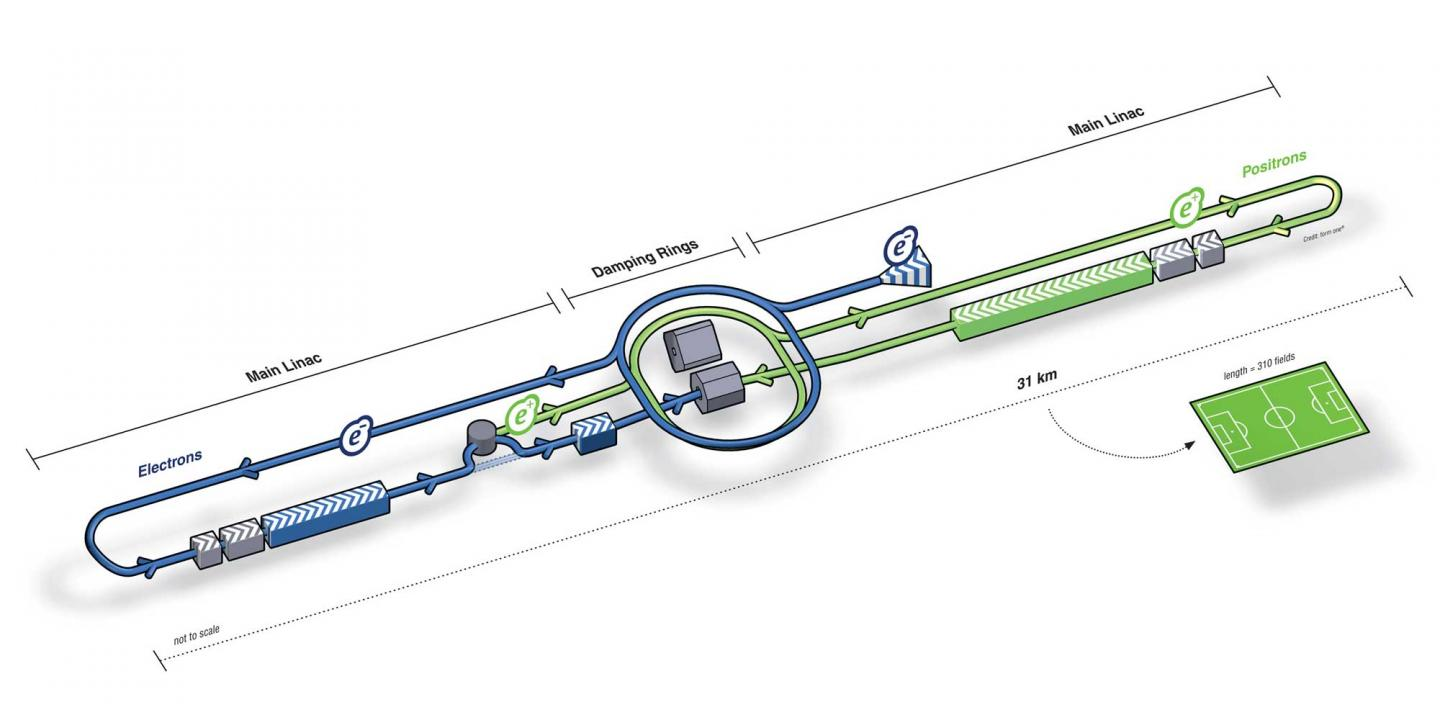
\includegraphics[width=\textwidth]{../img/ilc.jpg} 
	\caption{Schéma ILC\cite{cern:ilc}}
	\label{ilc:schema}
\end{figure}

L'objectif de l'ILC est de produire beaucoup de boson de Higgs, notamment pour découvrir s'il y en a d'autres générations du boson de Higgs. Et plus globalement pour rechercher de la nouvelle physique, par de nouveaux écarts avec le \MS.\\

À l'heure actuelle, ce projet attend les autorisations pour lancer sa construction, probablement dans les montagnes au nord du Japon. 
Et le détecteur SDHCAL correspond parfaitement aux spécifications nécessaires pour un accélérateur linéaire de ce type.
C'est pourquoi, afin de consolider sa candidature pour l'appel d'offre, l'IP2I développe aussi des programmes d'analyse de ce détecteur.

\section{Programme : \original}

% Contexte
Au début de mon stage, j'ai récupéré les codes de Guillaume \textsc{Garillot}, qui les a développé en 2021 au cours de son post-doctorat à l'IP2I. 

Son projet se divise en 3 programmes indépendants \Figure{\ref{orga:init}} :

\begin{description}
	
	\item[\texttt{miniDSTMarker}] qui permet de récupérer les données\footnote{aujourd'hui simulées mais plus tard obtenues dans le détecteur} sur le serveur distant où elles sont stockées.
	
	\item[\texttt{processor}] permet de tirer, des données brutes précédentes, des arbres \ROOT s.
	
	\item[\texttt{analysis}] utilise les méthodes des arbres binaires boostés pour effectuer une analyse statistique des arbres \ROOT issus du programme \texttt{processor}.
	
\end{description} 

% Organisation du projet initial : https://github.com/ggarillot/nnhAnalysis/tree/refactor

\begin{figure}[!ht]
	\centering
	\begin{tikzpicture}

		\tikzstyle{home}=[draw, rectangle, fill=red!50, text=black, rounded corners=3pt]		
		
		\tikzstyle{directory}=[draw, rectangle, fill=gray!30, text=black, rounded corners=3pt]

		\node[home] (A) at (0,0) {\texttt{nnhAnalysis}};
		
		\node[directory] (AM) at (-4,-2.5){\minidstmarker};
		\node[directory] (AP) at (0,-2.5) {\processor};
		\node[directory] (AA) at (4,-2.5) {\analysis};
		
		
		\tikzstyle{linkDir}=[->,dotted,very thick,>=latex]
		
		\draw[linkDir] (A)--(AM);
		\draw[linkDir] (A)--(AP); 
		\draw[linkDir] (A)--(AA);
		
	\end{tikzpicture}
	\caption{
		Organisation des dossiers de mon Projet - \url{https://github.com/ggarillot/nnhAnalysis/tree/refactor}
	}
	\label{orga:init}
\end{figure}

En résumer, ce projet permet l'analyse des collisions survenues dans ce détecteur pour le projet ILC.


\subsection{Données initiales}

% données distantes : 

Malheureusement, pour le temps de ce stage, je n'ai pas obtenu l'accès au serveur, donc je n'ai pas pu utilisé \texttt{miniDSTMarker}. Je l'ai donc pas testé, ni pu développer ma propre version. C'est pourquoi, j'ai décidé de ne pas l'inclure dans mon propre code.\\

% données locales
Pour que je puisse travailler, on a mis à ma disposition certains de quelqu'un de ces fichiers, ceux des collisions à 250 $\GeV$. Soient 66 dossiers \Figure{\ref{data:list}} de fichiers \LCIO, où chaque nom correspond au code du type de processus \Figure{\ref{data:def}}.

\begin{figure}[h!]
	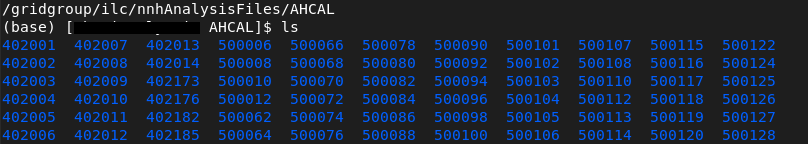
\includegraphics[width=\textwidth]{../img/listeProcessus.png} 
	\caption{Les noms des dossiers correspondent aux numéros de processus}
	\label{data:list}
\end{figure}

% Tableau des codes associés aux résultats des processus

\begin{figure}[h!]
    \centering
    \begin{tabular}{ | l | l | l | }
    		\hline
    		Type de processus & Code des processus \\
        \hline
        2 leptoniques & 500006, 500008 \\
        \hline
        2 hadroniques & 500010, 500012 \\
        \hline
        4 hadroniques & 500062, 500064, 500066, 500068, 500070, 500072 \\
        \hline
        4 semi-leptoniques & 500074, 500076, 500078, 500080, 500082, 500084, 500101, 500102, 500103, 500104, \\ 
        & 500105, 500106, 500107, 500108, 500110, 500112 \\
        \hline
        4 leptoniques & 500086, 500088, 500090, 500092, 500094, 500096, 500098, 500100, 500113, 500114, 500115, \\
        & 500116, 500117, 500118, 500119, 500120, 500122, 500124, 500125, 500126,500127, 500128  \\
        	\hline
        signal & 402007, \color{red}{402173}, \color{blue}{402176}\\
        \hline
        autres higgs & 402001, 402002, 402003, 402004, 402005, 402006, 402008, 402009, 402010, 402011, 402012, \\ 
        & 402013, 402014, 402182, 402185, \color{blue}{402173}, \color{red}{402176}\\
        \hline
    \end{tabular}
    \caption{Signification des codes des processus, \color{red}{si le signal recherché est de type \bb}, \color{blue}{si le signal est \WW}}
    \label{data:code}
\end{figure}

%if (isBB) 
%        CHANNELS_SIGNAL.insert(402173);
%        CHANNELS_OTHERHIGGS.insert(402176);
%else 
%        CHANNELS_SIGNAL.insert(402176);
%        CHANNELS_OTHERHIGGS.insert(402173);

\subsection{Conversion des fichiers initiaux en fichiers \ROOT}

Grâce au programme \processor on va pouvoir convertir les fichiers initiaux \SLCIO en fichiers \ROOT standards, afin de pouvoir les analyser.\\

On obtient ainsi pour chaque dossier de fichier de données \SLCIO un fichier \ROOT en sortie, \cad que l'on obtiendra un arbre \ROOT par type de processus.\\

Ce programme doit être robuste et donc à partir des mêmes fichiers d'entrées toujours générer des fichiers \ROOT strictement identiques.

\subsection{Analyses des collisions}

\subsubsection{Étape 1}

Avant de commencer l'analyse des fichiers \ROOT générés précédemment, on va terminer ce que le programme \processor avait commencé, et fusionner l'intégralité de ces fichiers en un seul gros fichier \texttt{DATA.root}, grâce à la commande \texttt{hadd}. 
Cette commande a été développé par le CERN et elle fusionne tous les histogrammes de différents fichiers en un seul\cite{root:hadd}. 

Donc là encore, la répétition de ce programme doit toujours générer des fichiers \texttt{DATA.root} strictement identique.

\subsubsection{Étape 2}

Pour la deuxième étape de ce programme \analysis, on va trier nos données en 4 fichiers distincts. 
Mais au lieu de les séparer par leur numéro de processus, qui est un critère numérique donc éloigné de la réalité des résultats d'une véritable expérience, on va les diviser suivant la polarisation initiale des particules incidentes, \cad l'électron et le positron à -0,8 et 0,3 ou les 2 nulles. 
Et par le type de particules produites par un boson de Higgs, \cad les canaux \bb et \WW, puisque ce sont les plus probables\footnote{Rien n'empêchera d'ajouter d'autres canaux même si le code manque encore de un peu de modularité.}.

\begin{figure}[h!]
	\centering
	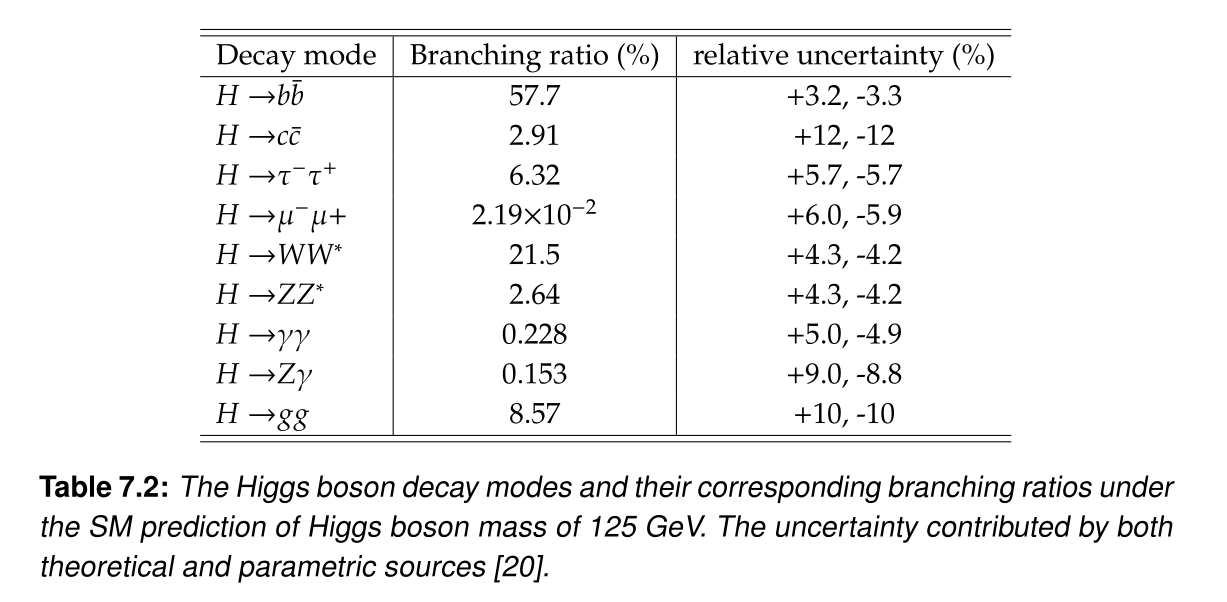
\includegraphics[width=\textwidth]{../img/Higgs_decay_125GeV.png} 
	\caption{
		Les modes de désintégrations du boson de Higgs à 125 $\GeV$
		\cite{liu:tel-03405418}.
	}
\end{figure}

Donc on obtient ces 4 fichiers suivants :

% Fichiers "split"

%\begin{figure}[h!]
%	\centering
%	\begin{lstlisting}
%			split_bb_e-0.8_p+0.3.root
%			split_bb_e+0_p+0.root
%			split_ww_e-0.8_p+0.3.root
%			split_ww_e+0_p+0.root
%	\end{lstlisting}
%	\label{files:split}
%	\caption{Fichiers où les évènements sont séparés en fonction des caractéristiques des polarisations des particules incidentes et des types de particules résultantes.}
%\end{figure}

\begin{figure}[h!]
	\centering
	\begin{tabular}{ | c | c | c | c | }
		\hline
		Polarisation & \multicolumn{2}{c|}{Canal} \\
		\hline
		$(e,p)$ & \bb &  \WW \\
		\hline
		$(0,0)$ & \verb|split_bb_e+0_p+0.root| & \verb|split_ww_e+0_p+0.root| \\
		\hline \cline{2-3}
		$(-0.8, +0.3)$ & \verb|split_bb_e-0.8_p+0.3.root| & \verb|split_ww_e-0.8_p+0.3.root| \\
		\hline
	\end{tabular}
	\label{files:split}
	\caption{Tous les évènements sont séparés en 4 fichiers suivant la polarisation des particules incidentes et des types des particules produites par le boson de Higgs.}
\end{figure}

Dans chacun de ces fichiers les arbres \ROOT, \texttt{TTree}, auront les variables suivantes :

\begin{description}

	\item[\texttt{isSignal} :] booléen qui indique si on considère l'évènement comme du signal ou du bruit de fond.
	
	\item[\texttt{channelType} :] entier qui représente le type de canaux de l'évènement \Figure{\ref{data:code}}:
	\begin{itemize}
		\item 2 fermions leptoniques ou hadroniques
		\item 4 fermions leptoniques ou semi-leptoniques ou hadroniques 
		\item une autre type de résultat avec un boson de Higgs
	\end{itemize}
	
	\item[\texttt{isTrain}] booléen qui confirme si l'évènement a été entrainé ou testé par la BDT.
	
	\item[\texttt{preSelected}] booléen, si l'évènement a été pré-sélectionné par la BDT.
	
	\item[\texttt{weight}] flottant qui est le poids de l'évènement en $fb^{-1}$ de la luminosité intégrée.
	
\end{description}


Pour trier les données du fichier \texttt{DATA.root}, on va utiliser des BDT pour \textit{Boosted Decision Tree}, en français, des arbres de décision boostés. 

Les arbres sont des structures de données courantes en informatique, ils sont utilisées notamment pour trier les données car ils ont une rapidité optimale en temps. 
Ici on utilise les arbres pour déterminer la nature des particules en répondant à des questions booléennes (Similaire à l'exemple \Figure{\ref{ExampleBDT}}. Et comme il n'y a que 2 issus à chaque nœud, on parle d'arbre binaire. 

\begin{figure}[h!]
	\center
	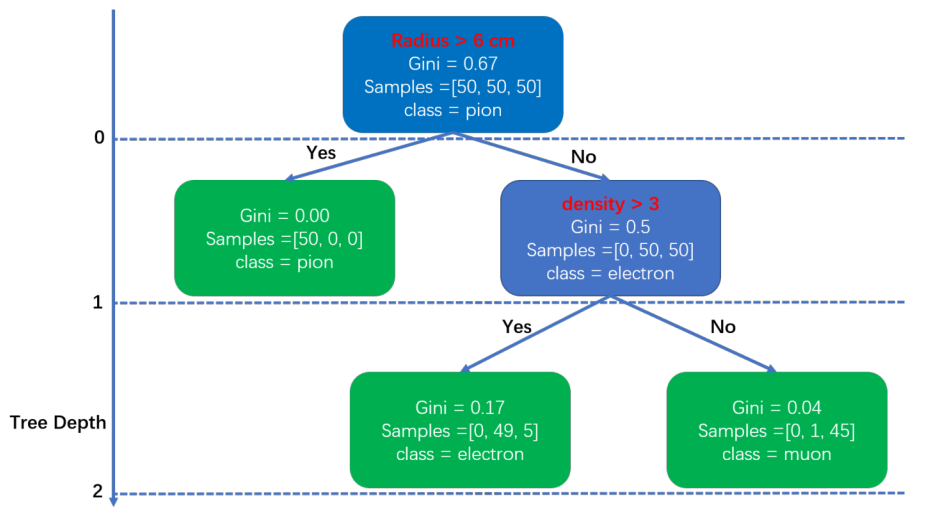
\includegraphics[width=\textwidth]{../img/ExampleBDT.png}
	\caption{Exemple de BDT \cite{liu:tel-03405418}. Ici, elle permet de déterminer de le type d'une particule}
	\label{ExampleBDT}
\end{figure}

Une fois encore, des méthodes ont déjà été développé dans l'API du CERN\cite{root:treeFriend}. Ces méthodes utilisent des paramètres générées aléatoirement afin d'augmenter la rapidité des calculs. C'est pourquoi on parle d'arbre boosté.

Mais cette fois-ci les fichiers créés sont équivalents mais pas identique. Car les BDT utilisent la génération de nombre aléatoire, ce qui engendre des variations dans les entraînements.

\subsubsection{Étape 3}

Et pour terminer, on peut enfin effectuer l'analyse à proprement parlé de nos données à partir des fichiers \texttt{split\_XX.root} précédents \Figure{\ref{files:split}}.

Cette étude se fait sur les fichiers avec une polarisation non nulle pour les particules incidentes. Car \doToList{????}


% Fichiers "model"

%\begin{figure}[h!]
%	\centering
%	\begin{lstlisting}
%			model_bb_e-0.8_p+0.3.joblib
%			model_ww_e-0.8_p+0.3.joblib
%	\end{lstlisting}
%	\caption{Fichiers du model de la BDT}
%	\label{files:model}
%\end{figure}

\begin{figure}[h!]
	\centering
	\begin{tabular}{ | c | c | c | c | }
		\hline
		Polarisation & \multicolumn{2}{c|}{Canal} \\
		\hline
		$(e,p)$ & \bb &  \WW \\
		\hline \cline{2-3}
		$(-0.8, +0.3)$ & \verb|model_bb_e-0.8_p+0.3.joblib| & \verb|model_ww_e-0.8_p+0.3.joblib| \\
		\hline
	\end{tabular}
	\label{files:model}
	\caption{Fichiers du model de la BDT.}
\end{figure}
	
% Fichiers "scores"

%\begin{figure}[h!]
%	\centering
%	\begin{lstlisting}
%			scores_bb_e-0.8_p+0.3.root
%			scores_ww_e-0.8_p+0.3.root
%	\end{lstlisting}
%	\caption{Les fichiers scores ont la réponse de la BDT : 2 variables pour chaque évènement, un booléen pour savoir s'il est sélectionné et la valeur retournée par la BDT}
%	\label{files:scores}
%\end{figure}

\begin{figure}[h!]
	\centering
	\begin{tabular}{ | c | c | c | c | }
		\hline
		Polarisation & \multicolumn{2}{c|}{Canal} \\
		\hline
		$(e,p)$ & \bb &  \WW \\
		\hline \cline{2-3}
		$(0,0)$ & \verb|scores_bb_e-0.8_p+0.3.root| & \verb|scores_ww_e-0.8_p+0.3.root| \\
		\hline
	\end{tabular}
	\label{files:scores}
	\caption{Les fichiers scores ont la réponse de la BDT : 2 variables pour chaque évènement, un booléen pour savoir s'il est sélectionné et la valeur retournée par la BDT.}
\end{figure}

% Fichiers "bestSelection"

%\begin{figure}[h!]
%	\centering
%	\begin{lstlisting}
%			bestSelection_bb_e-0.8_p+0.3.root
%			bestSelection_ww_e-0.8_p+0.3.root
%	\end{lstlisting}
%	\caption{
		%Ce fichier \ROOT contient tous les arbres \texttt{TTree} 
		%sélectionnés par la BDT comme un évènement \nnh donne 
		%$b \bbar$ ou $W \Wstar$
%	}
%	\label{files:bestSelection}
%\end{figure}

\begin{figure}[h!]
	\centering
	\begin{tabular}{ | c | c | c | c | }
		\hline
		Polarisation & \multicolumn{2}{c|}{Canal} \\
		\hline
		$(e,p)$ & \bb &  \WW \\
		\hline
		\hline \cline{2-3}
		$(-0.8, +0.3)$ & \verb|bestSelection_bb_e-0.8_p+0.3.root| & \verb|bestSelection_ww_e-0.8_p+0.3.root| \\
		\hline
	\end{tabular}
	\label{files:bestSelection}
	\caption{Ce fichier \ROOT contient tous les arbres \texttt{TTree} 
		sélectionnés par la BDT comme un évènement de \texttt{nnh}}
\end{figure}

% Fichiers "stats"

%\begin{figure}[h!]
%	\centering
%	\begin{lstlisting}
%			stats_bb_e-0.8_p+0.3.joblib
%			stats_ww_e-0.8_p+0.3.joblib
%	\end{lstlisting}
%	\caption{Statistiques.}
%	\label{files:stats}
%\end{figure}

\begin{figure}[h!]
	\centering
	\begin{tabular}{ | c | c | c | c | }
		\hline
		Polarisation & \multicolumn{2}{ c | }{Canal} \\
		\hline
		$(e,p)$ & \bb &  \WW \\
		\hline \cline{2-3}
		$(-0.8, +0.3)$ & \verb|stats_bb_e-0.8_p+0.3.joblib| & \verb|stats_ww_e-0.8_p+0.3.joblib| \\
		\hline
	\end{tabular}
	\label{files:stats}
	\caption{Fichiers des résultats statistiques pour les polarisations des particules incidentes à 0,8 pour l'électron et à 0,3 pour le positron.}
\end{figure}

Et même si cette analyse sera toujours la même \qqs les fichiers \texttt{split\_XX.root}, ces derniers étant légèrement différent d'un entraînement à l'autre les résultats statistiques \Figure{\ref{files:stats}} seront, là encore, légèrement différent mais doivent rester équivalent.

\section{Programme : \ilcsoft}

À présent, je vais vous présenter les modifications que j'ai apporté au programme \original.

Dans un premier temps, j'ai fais de la cosmétique : j'ai typé les variables, appliqué les bonnes règles de typographie et commenté les différents fichiers, classes, interfaces, fonctions, et variables globales. Ce qui m'a permis de bien comprendre les programmes et de le rendre plus lisible pour les futurs développeurs de ce code.

Ensuite je les ai modifié pour qu'il puisse s'exécuter en parallèle. En effet, \processor et \analysis mettent quelques heures à s'exécuter. Et pour tester leurs robustesses et pouvoir faire des statistiques, il est nécessaire de le faire de très nombreuses fois. Donc cette nouvelle fonctionnalité la version \ilcsoft permet un gain de temps considérable. Et plus tard, cela permettra aussi d'exécuter avec différents jeux de données (niveaux d'énergies, canaux...).

\subsection{Données}

Donc bien sûr, il s'agit des mêmes fichiers \SLCIO que pour le programme \original \Figure{\ref{data:list}}

\subsection{Programme : \processor}

Le but est toujours la conversion de chaque dossier de fichiers \SLCIO en un seul fichier \ROOT.

Pour aider à la lisibilité du programme, j'ai aussi développé une nouvelle classe qui permet de simplifier sa lecture.
Ma classe \texttt{PDGInfo} permet de manipuler plus facilement les outils du PDG, grâce à une correspondance entre les codes entiers des particules et leurs noms, ainsi que quelques méthodes et tests booléennes\footnote{\url{https://github.com/alexhxia/nnhAnalysis/blob/main/nnhProgram/ilcsoft/processor/include/PDGInfo.hh}}.

\subsection{Programme : \analysis}

La encore le fonctionnement global reste inchangé, par rapport à \original

\chapter{Programme \texttt{FCC}}

\section{Présentation du Projet FCC}

Le FCC (Futur Collisionneur Circulaire) est le projet du CERN pour remplacer 
leur collisionneur actuelle, le LHC (Large Hadronic Collider). 
Dont la fin de l'exploitation est prévu en 2040 \cite{cern:fcc}.
On prévoit un anneau de 100 km, contre 27 km pour le LEP et le LHC 
(comme montrer Figure~\ref{fcc:img}).
Ce qui devrait nous permettra d'atteindre une énergie de 100 $\TeV$ contre 13 $\TeV$
actuellement pour le LHC.

L'objectif est la rechercher d'une nouvelle physique par la mise en évidence de déviation avec le modèle standard. Et plus particulièrement, en augmentant la statistique sur le boson de Higgs, découvert avec le collisionneur actuelle, afin de mieux comprendre sa physique.

\begin{figure}[!ht]
    \centering
    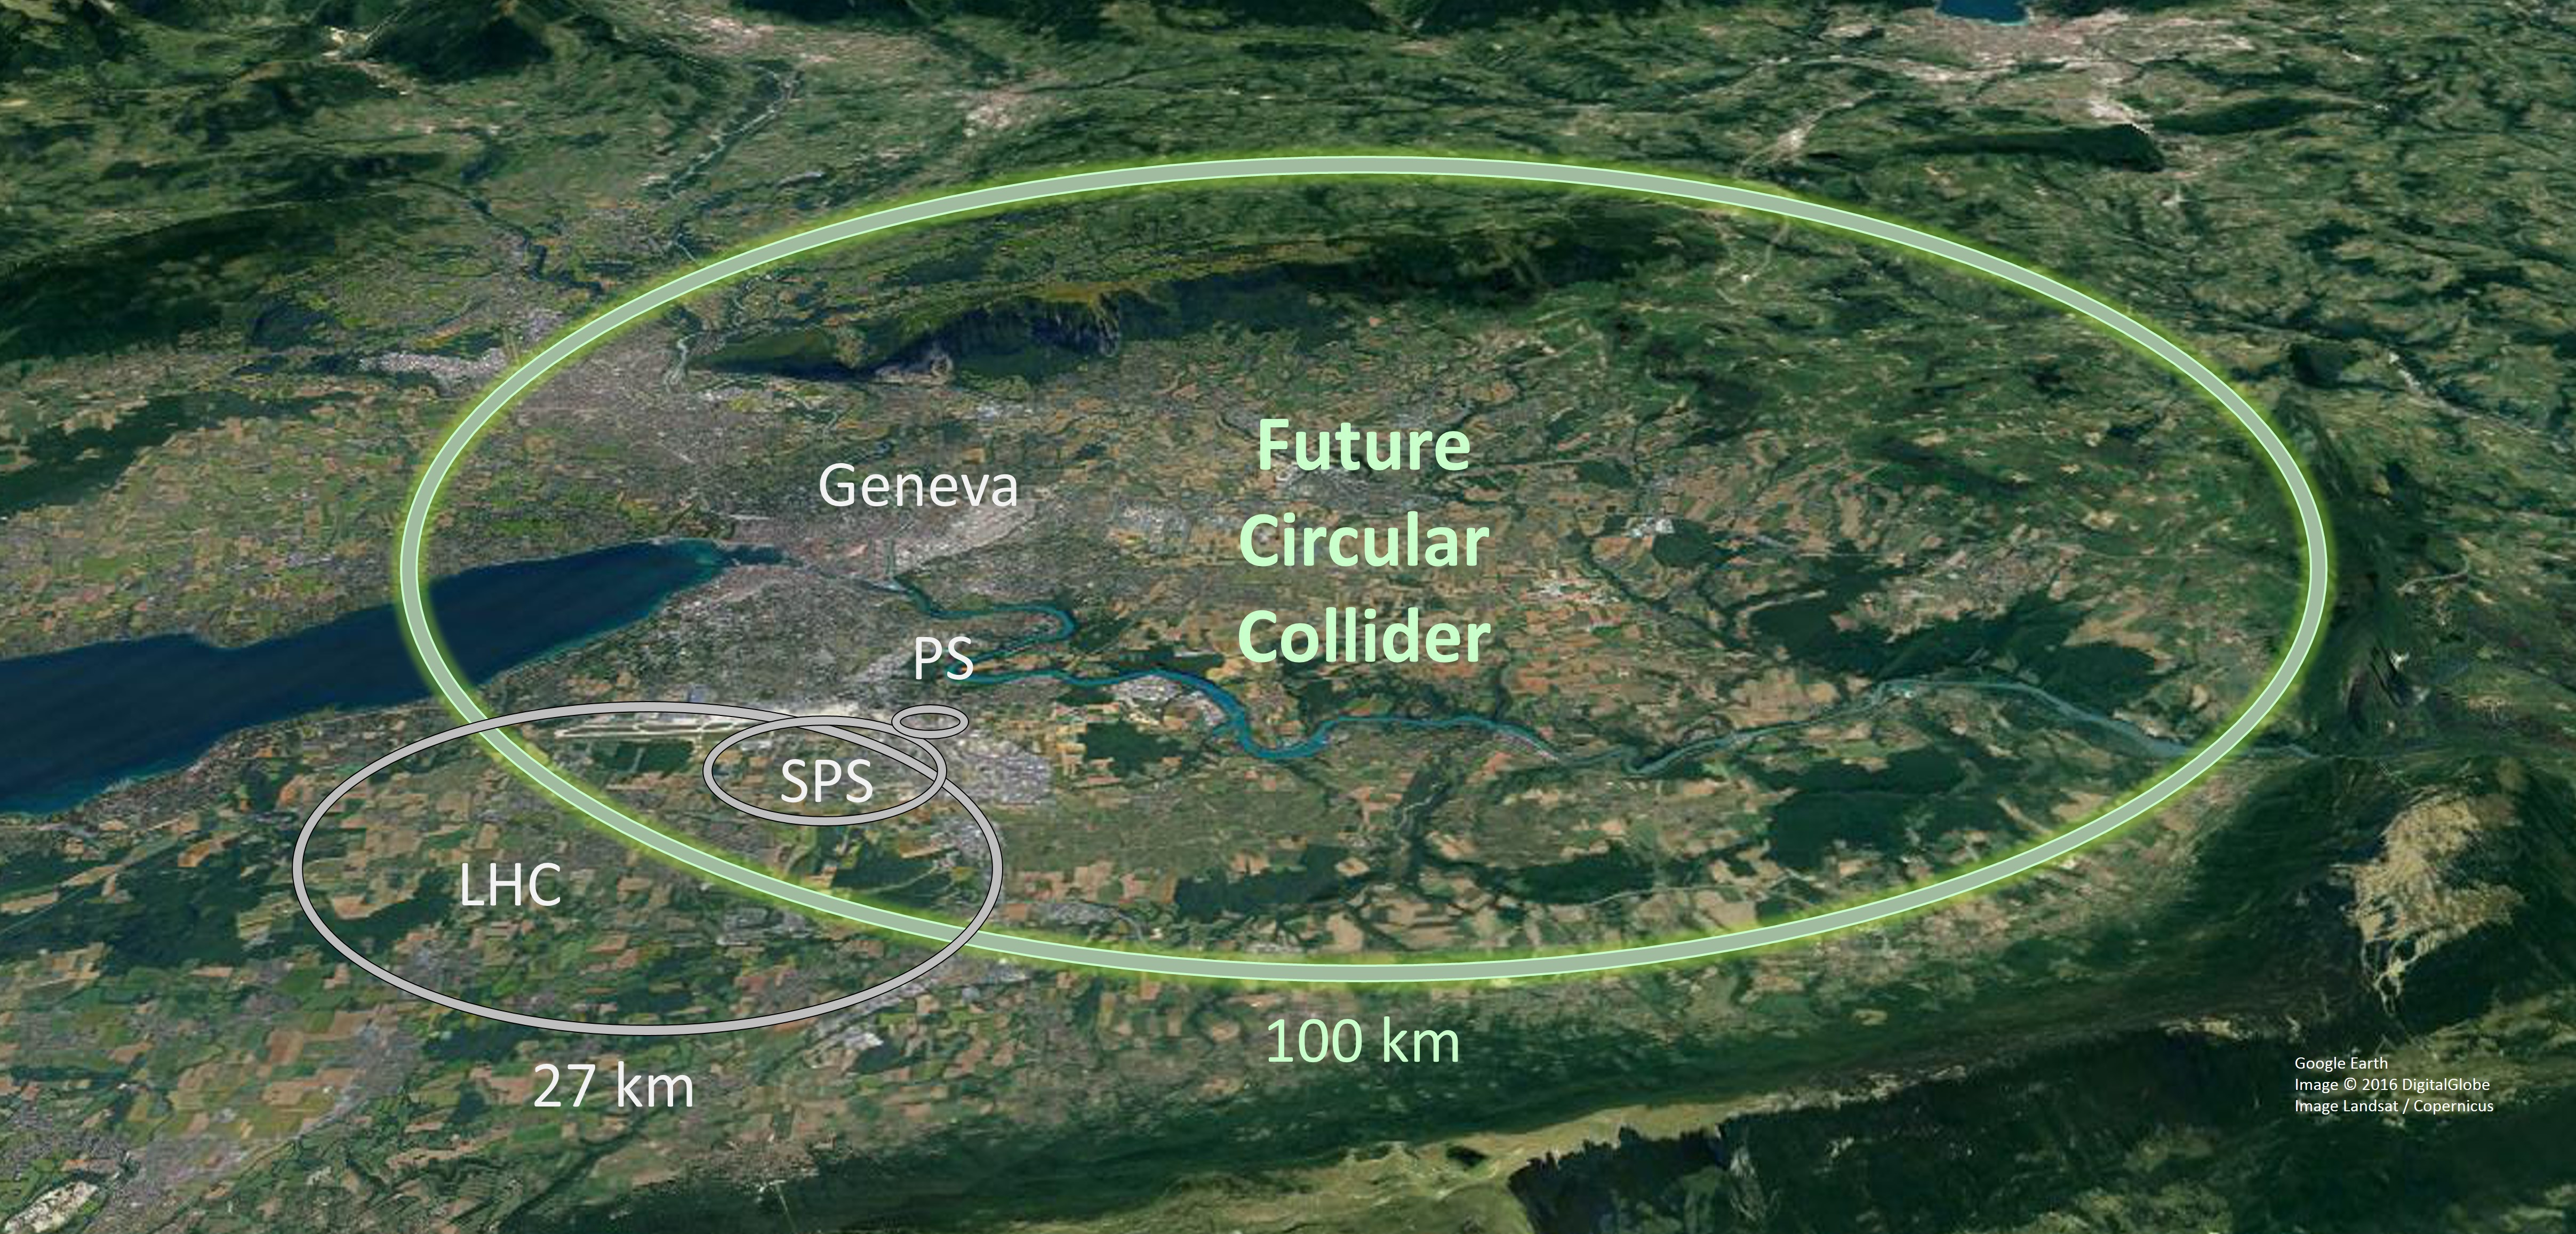
\includegraphics[width=\textwidth]{../img/FCC.jpg}
    \caption{https://cds.cern.ch/images/OPEN-PHO-ACCEL-2019-001-2}
    \label{fcc:img}
\end{figure}

Une fois encore, le détecteur SDHCAL candidate pour ce projet et pourrait être y être installer.

\section{Développement Numérique}

Mon objectif est d'adapter les codes développés précédemment par Guillaume 
\textsc{Garillot} du projet ILC au projet FCC qui n'utilise pas les mêmes suites logiciels.


\subsection{Programme : \convert}

Dans un premier temps, je dois convertir les fichiers \SLCIO en fichiers \ROOT en utilisant le programme libre \texttt{k4MarlinWrapper} du projet de \texttt{key4hep}\footnote{\url{https://github.com/key4hep/k4MarlinWrapper}}. 
Il s'agit d'une collaboration entre chercheurs du CERN dont l'objectif est de développer des outils pour le projet FCC, y compris des utils de conversion entre \LCIO (\iLCSoft) et \EDMhep (\FCC).%, en utilisant les algorithmes \texttt{Gaudi}
\\

Cette partie a été laborieux, car le programme \texttt{k4MarlinWrapper} est en cours de développement. 
J'ai du faire remonter de très nombreux problèmes en parallèle de mon travail. 
En effet, à chaque mise à jour, le programme ne fonctionnait plus, ce qui m'a fait perdre beaucoup de temps en essayant de comprendre le problème, le signaler et le corriger quand je le comprenais, ou patienter pour que quelqu'un d'autre le corrige. 

\subsection{Programme : \processor}

Comme les fichiers d'entrées sont à présent des fichiers \ROOT, il faut adapter cette partie pour que les fichiers de sortie soit les mêmes ou au moins équivalent.

\subsection{Programme : \analysis}

Cette partie reste inchangé par rapport à \ilcsoft.
% Outils Numériques


\chapter{Outils Numériques}

Pour utiliser et comparer les résultats obtenus facilement, j'ai développé de très nombreux programmes supplémentaires afin de pouvoir automatiser leur utilisation, mais aussi de les exécuter sur un serveur distant. 

\section{Répertoire \texttt{script}}

Dans ce dossier\footnote{\url{https://github.com/alexhxia/nnhAnalysis/tree/main/script}}, j'ai développé des outils d'automatisation de l'exécution des programmes. En effet, avant pour lancer un \processor ou une \analysis il y avait de très nombreuses commandes à taper au terminal et parfois incompatible entre elles.
J'ai donc développé 6 programmes principaux d'automatisation des programmes :

\begin{description}
	
	\item[\texttt{nnh}]	programme générale qui permet l'exécution de tout le programme (\convert, \processor et \analysis) et plusieurs fois.
	\begin{description}

	\item[\texttt{nnhConvert}] permet de convertir les fichiers \SLCIO en fichiers \ROOT.
	
	\item[\texttt{nnhProcessor}] d'exécuter tout le programme \processor.
	
	\item[\texttt{nnhAnalysis}] exécute tout le programme \analysis.
	
	\begin{description}
		
		\item[\texttt{prepareBDT}] exécute la préparation de la BDT.
		
		\item[\texttt{launchBDT}] lance la BDT \footnote{Le programme \texttt{launchBDT} est incompatible avec les autres, ce qui nécessite de le lancer dans un terminal enfant.}.
		
	\end{description}
	\end{description}
	
\end{description}

Chacun de ces programmes peuvent être lancé ensemble mais aussi séparément. Ce qui permet de gagner énormément en temps d'utilisation mais aussi de pouvoir personnaliser selon les besoins de l'utilisateur.

\section{Répertoire \texttt{test}}

Pour tester les résultats obtenus, j'ai développé 4 programmes en \texttt{python}.  Et de tester s'ils sont compatibles entre eux.

\begin{figure}[h!]
	\center
	\begin{tabular}{| c | c | c |}
		\hline
			\texttt{•} & \texttt{Processus} & \texttt{Analysis} \\
		\hline
			\texttt{Completed} & \texttt{testProcessorCompleted.py} & \texttt{testAnalysisCompleted.py} \\
		\hline
			\texttt{Same} & \texttt{testProcessorSame.py} & \texttt{testAnalysisSame.py} \\
		\hline
	\end{tabular}
	\caption{Tableau récapitulatif des fonctions de tests}
\end{figure}

\subsection{Programmes \texttt{testXxCompleted.py}}

L'objectif de ce type de programme est de tester si tous les fichiers qui aurait du être créer, l'ont bien été. Ces programmes sont très rapides, ne prennent que en quelques secondes.

Ce qui permet, en cas de problèmes de relancer juste la partie qui n'est pas terminé et pas tout le programme.

\subsubsection{Programmes \texttt{testProcessorCompleted.py}}

Un \processor est complet si tous les dossiers du répertoire d'entré (\Figure{\ref{data:list}}) ont bien généré un fichier \ROOT.

\subsubsection{Programmes \texttt{testAnalysisCompleted.py}}

Une \analysis est complète si elle contient 13 fichiers, car :
\begin{description}
	\item[hadd :] 1 fichier \verb|data.root|
	\item[prepareBDT :] 4 fichiers (2 polarisations $\times$ 2 canaux) \verb|split_XX.root| 
	\item[launchBDT :] 2 fichiers (2 canaux) \verb|model_XX.joblib|, \verb|scores_XX.root|, \verb|bestSelection_XX.root|, \verb|stats_XX.json|
\end{description}

\subsection{Programmes \texttt{testXxSame.py}}

Ce type de programme\footnote{\url{https://github.com/alexhxia/nnhAnalysis/tree/main/test}
} va prendre quelques dizaines de minutes à une heure pour s'exécuter, car il va comparer tous les arbres \ROOT des différents fichiers pour s'assurer que 2 fichiers sont identiques ou au moins compatibles. Cette comparaison se ferait avec la fonction de Kolmogorov présente, là encore, dans l'API du CERN, qui compare 2 histogrammes et retourne un flottant sur leur compatibilité. Dans le chapitre \original, j'ai explicité que les programmes qui donnaient des résultats toujours identiques et ceux qui devaient avoir des résultats équivalents. 

\subsubsection{Programmes \texttt{testProcessorSame.py}}

Toutes les exécutions de \processor doivent donner des résultats identiques, surtout au sein du même projet. Et j'ai pu le confirmer en comparant plusieurs résultats obtenus de différentes exécutions. 

Et lorsque j'ai apporté des corrections au programme, quand je suis passée de \original à \ilcsoft, cela m'a permis de vérifier que mon code obtenait bien le même résultat. De même, de \ilcsoft à \fcc.

\subsubsection{Programmes \texttt{testAnalysisSame.py}}

La comparaison entre 2 exécutions du programme \analysis est plus compliquée, puisque la BDT utilise des nombres aléatoires, ce qui ne permet pas d'obtenir des résultats identiques.

Certains fichiers doivent rester identiques comme les fichiers \verb|data.root| ou \verb|split_XX.root|. Certains sont complètement différents comme les fichiers \verb|model_XX.joblib| ou \verb|bestSelection_XX.root|, car ils sont liés à l'entraînement de la BDT. Mais à la fin les fichiers \verb|stat_XX.json| doivent être statistiquement compatibles.

\subsection{Répertoire \texttt{result}}

Dans ce répertoire, je place les fichiers de sorti des programmes \texttt{test}. 
En effet, quand on exécute un programme de test, l'utilisateur a la possibilité d'obtenir les résultats sous la forme d'un fichier \texttt{JSON}. 
Ce qui permet d'en garder une trace et de ne pas refaire un test déjà effectué.\\

\subsection{Mes résultats}

Je peux donc confirmer que mes programmes s'exécutent complètement, correctement et avec des écarts statistiques faibles aux finals (générés par l'utilisation de BDT).

%%%%%%%%%%%%%%%%%%%%%%%%%%%%%

\chapter{Résultats Physiques}

\section{Résultats Numériques}

Les résultats de l'étude statistique sont dans les fichiers de type \verb|stats_XX.json|, et sont triés suivant 10 catégories. 

\begin{figure}[!ht]
	\centering
	\begin{subfigure}[b]{0.45\textwidth}
		\begin{description}
			\item[0] \verb|Signal|
			\item[1] \verb|Other higgs->WW*|
			\item[2] \verb|Other higgs|
			\item[5] \verb|2 fermions leptonic|
			\item[6] \verb|2 fermions hadronic|
			\item[8] \verb|4 fermions hadronic|
			\item[9] \verb|4 fermions semileptonic|
			\item[7] \verb|4 fermions leptonic|
		\end{description}
		\label{stats:results:WW}
		\caption{Pour le canaux \WW}
	\end{subfigure}
     \hfill
	\begin{subfigure}[b]{0.45\textwidth}
		\begin{description}
			\item[0] \verb|Signal|
			\item[3] \verb|Other higgs->bb|
			\item[4] \verb|Other higgs|
			\item[5] \verb|2 fermions leptonic|
			\item[6] \verb|2 fermions hadronic|
			\item[8] \verb|4 fermions hadronic|
			\item[9] \verb|4 fermions semileptonic|
			\item[7] \verb|4 fermions leptonic|
		\end{description}
		\caption{Pour le canaux \bb}
		\label{stats:results:bb}
	\end{subfigure}
	\label{stats:results}
	\caption{Les numéros et les noms des différentes catégories d'\analysis pour l'étude statistique}
\end{figure}

Et dans chaque catégorie, plusieurs variables sont calculées \Figure{\ref{stats:results:vrb}}.

\begin{figure}[!ht]
	\centering
	\begin{description}
		\item[\texttt{name}] nom du type de l'évènement, 
				cité dans \Figure{\ref{stats:results}}
		\item[\texttt{stat}] nombre total d'évènement mesuré
		\item[\texttt{sum}] somme des poids de chaque évènement (signal sur bruit)
		
		\item[\texttt{statPreSel}] nombre d'évènement pré-sélectionnés par la BDT
		\item[\texttt{effPreSel}] taux de pré-sélection
		\item[\texttt{sumPreSel}] somme des poids des évènements pré-sélectionnés 
		
		\item[\texttt{effSel}] taux de sélection
		\item[\texttt{sumSel}] somme des poids des évènements sélectionnés
	\end{description}
	\caption{Variables statistiques de chacune des catégories précédentes \Figure{\ref{stats:results}}}
	\label{stats:results:vrb}
\end{figure}

\subsection{Partie \original}

Regardons 2 résultats d'\analysis différents pour \bb, dans le cas d'un signal \Figure{\ref{stats:results:img}} :

\begin{figure}[!ht]
	\centering
	\begin{subfigure}[b]{0.45\textwidth}
		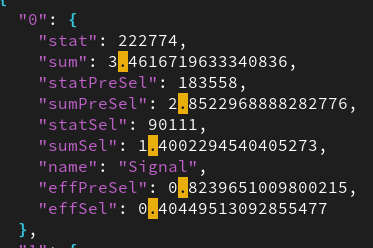
\includegraphics[width=\textwidth]{../img/stats_bb_original_run1_run1.png} 
		\label{stats:results:bb:original:1:1}
		\caption{Canal \bb, branche \original, run 1}
	\end{subfigure}
     \hfill
	\begin{subfigure}[b]{0.45\textwidth}
		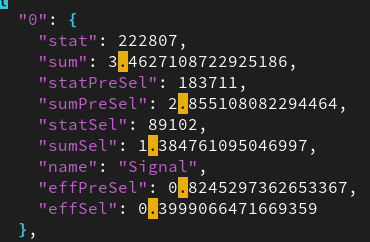
\includegraphics[width=\textwidth]{../img/stats_bb_original_run2_run1.png}
		\caption{Canal \bb, branche \original, run 2}
		\label{stats:results:bb:original:2:1}
	\end{subfigure}
	\label{stats:results:img}
	\caption{Les numéros et les noms des différentes catégories d'\analysis pour l'étude statistique}
\end{figure}

On constate un écart initial sur le nombre d'évènement de moins de 0.01\%, puis une diminution des évènements pré-sélectionnés de 17,6\% pour le \textit{run 1} contre 17,5\% pour le \textit{run 2}. Et une diminution de 59,6\% et 60,0\% pour les évènements sélectionnés par la BDT. 

L'autre constat est qu'on subit une grosse diminution entre les variables \texttt{sum} et \texttt{effSel}, de 88,3\% et 88,5\%, ce qui traduit une baisse importante de luminosité induit par le signal, une fois débarrassée du bruit de fond. Mais une fois encore ces résultats sont cohérents. \\

Donc même si les résultats sont proches, ils ne sont pas identiques puisque la BDT utilise des nombres aléatoires dans sa prise de décision sur le type d'évènement. Mais le programme reste robuste, et que l'utilisation d'une BDT n'est pas une solution idéale puisqu'elle induise une incertitude numérique supplémentaire.


\section{Physique du Higgs}

\subsection{Section efficace}

\subsubsection{Quelques constantes}
Avant de commencer, je vais rappeler certaines constantes utiles pour la suite tirée du PDG, \textit{Particle Data Group} 2022\cite{Workman:2022ynf} :
\begin{description}

	\item[$\gHWW$] : couplage du boson de Higgs et du boson W

	\item[$\GF$] : constante de couplage de Fermi
	\footnote{\url{https://pdg.lbl.gov/2021/tables/contents_tables.html}}
	$$ \frac{G_\mathrm{F}}{\left(\hbar c\right)^3} = 1,166\,378\,7(6) \times 10^{-5}\, \GeV^{-2} $$
	$$ (\hbar c)^2 = \vhc \, \GeV^2 \, \mathrm{mbarn} = \vhc \times 10^{-31} \, \mathrm{m}.\GeV^2 $$
	
	\item[$\mH$] : masse du boson de Higgs
	\footnote{\url{https://pdglive.lbl.gov/Particle.action?node=S126&init=0}}
	$$ m_\mathrm{H_0} = 125,25 \pm 0,17 \, \GeV $$
		
	\item[$m_W$] : masse du boson W
	\footnote{\url{https://pdglive.lbl.gov/Particle.action?node=S043&init=0}}
	$$ m_\mathrm{W} = 80,377 \pm 0,012 \, \GeV $$
	
	\item[$s$] : variable de Mandelstam
	$$ s = \left(p_1 + p_2\right)^2 = \left(p_{e} + p_{p}\right)^2 $$
	Mes données correspondent aux simulations à : 
	$$ \sqrt{s} = 250\, \GeV $$

		
\end{description}

%%%%%%%%%%%%%%%%%%%%%%%%%%%%%%%%%%%

\subsubsection{Fusion $W\Wstar$ \cite{desy}}

Comme on est à très haute énergie, on peut approximer que $ \sqrt{s} >> 2 \mW $ :

\begin{equation}
	\sigma_\mathrm{WW-fusion} \longrightarrow 
		\frac{\gHWW^2 \, \GF^2}{32 \, \pi^3}
		\left[
			\left(1 + \frac{\mH^2}{s}\right) \log\left(\frac{s}{\mH^2}\right)
			- 2 \left(1 - \frac{\mH^2}{s}\right)
		\right]
\end{equation}


\begin{align*}
	\sigma_\mathrm{WW-fusion}
		&\approx\frac{\gHWW^2 \, \GF^2}{32 \, \pi^3}
		\left[
			\left(1 + \frac{\mH^2}{s}\right) \log\left(\frac{s}{\mH^2}\right)
			- 2 \left(1 - \frac{\mH^2}{s}\right)
		\right]\\
		&=\gHWW^2\frac{(\hbar c)^6}{32 \, \pi^3}
		\left[\frac{\GF}{(\hbar c)^3}\right]^2
		\left[
			\left(1 + \frac{\mH^2}{s}\right) \log\left(\frac{s}{\mH^2}\right)
			- 2 \left(1 - \frac{\mH^2}{s}\right)
		\right]\\
		&=\gHWW^2\frac{(\vhc)^3}{32 \, \pi^3}
		\left[\vGF\right]^2
		\left[
			\left(1 + \frac{\vmH^2}{\vs^2}\right) \log\left(\frac{\vs^2}{\vmH^2}\right)
			- 2 \left(1 - \frac{\vmH^2}{\vs^2}\right)
		\right]\\
		&\approx \gHWW^2 \times (-6,0466389\times 10^{-15})
\end{align*}

%%%%%%%%%%%%%%%%%%%%%%%%%%%%%%%%%%%

\subsubsection{La largeur partielle pour $W\Wstar$ \cite{desy}}

\begin{equation}
	\Gamma\left(H\longrightarrow WW\right) = 
		\frac{\gHWW^2 \, \mH^3}{64 \, \pi \, \mW^2}
		\left(1 - \frac{4 \mW^2}{\mH^2} + \frac{12 \mW^4}{\mH^4}\right)
		\left(1 - \frac{4 \mW^2}{\mH^2}\right)^{1/2}
\end{equation}

\begin{align*}
	\Gamma\left(H\longrightarrow WW\right) 
	&= \gHWW^2
		\frac{\vmH^3}{64 \, \pi \, \vmW^2}
		\left(1 - \frac{4\times \vmW^2}{\vmH^2} + \frac{12\times \vmW^4}{\vmH^4}\right)
		\left(1 - \frac{4\times \vmW^2}{\vmH^2}\right)^{1/2}\\
	&= \gHWW^2 
\end{align*}

%%%%%%%%%%%%%%%%%%%%%%%%%%%%%%%%%%%

\subsubsection{La section efficace de production du Higgs}

\begin{equation}
	\sigma_\mathrm{production} = \sigma_\mathrm{WW-fusion} \times \Gamma\left(H\longrightarrow WW\right)
\end{equation}

\begin{align*}
	\sigma 
		&= \frac{\gHWW^2 \, \GF^2}{32 \, \pi^3}
		\left[
			\left(1 + \frac{\mH^2}{s}\right) \log\left(\frac{s}{\mH^2}\right)
			- 2 \left(1 - \frac{\mH^2}{s}\right)
		\right]
		\times 
		\frac{\gHWW^2 \, \mH^3}{64 \, \pi \, \mW^2}
		\left(1 - \frac{4 \mW^2}{\mH^2} + \frac{12 \mW^4}{\mH^4}\right)
		\left(1 - \frac{4 \mW^2}{\mH^2}\right)^{1/2} \\
	\sigma &= \gHWW^4 \frac{\GF^2}{32 \, \pi^4} \frac{\mH^3}{64 \, \mW^2}
		\left[
			\left(1 + \frac{\mH^2}{s}\right) \log\left(\frac{s}{\mH^2}\right)
			- 2 \left(1 - \frac{\mH^2}{s}\right)
		\right]
		\left(1 - \frac{4 \mW^2}{\mH^2} + \frac{12 \mW^4}{\mH^4}\right)
		\left(1 - \frac{4 \mW^2}{\mH^2}\right)^{1/2} \\
	\sigma \propto \gHWW^4
\end{align*}

%%%%%%%%%%%%%%%%%%%%%%%%%%%%%%%%%%%

\subsection{Nombre de Higgs attendu}

Le nombre d'évènement est :
\begin{equation}
^	\mathcal{N}_\mathrm{event} 
	= \mathcal{N}_\mathrm{signal} 
	+ \mathcal{N}_\mathrm{background}
\end{equation}

Or le nombre d'évènement détecté est :
\begin{equation}
	\mathcal{N}_\mathrm{detect} 
	= \mathcal{N}_\mathrm{event} \pm \sigma(\mathcal{N}_\mathrm{event})
	= \mathcal{N}_\mathrm{event} \pm \sqrt{\mathcal{N}_\mathrm{event}}
\end{equation}

Et le signal est :
\begin{equation}
	\mathcal{N}_\mathrm{signal} 
	= \mathcal{N}_\mathrm{detect} 
	- \mathcal{N}_\mathrm{background}
\end{equation}

Donc le signal est :
\begin{equation}
	\mathcal{N}_\mathrm{detect} 
	- \mathcal{N}_\mathrm{background} 
	- \sqrt{\mathcal{N}_\mathrm{évènement}}
	\leq \mathcal{N}_\mathrm{signal} \leq
	\mathcal{N}_\mathrm{detect} 
	- \mathcal{N}_\mathrm{background} 
	+ \sqrt{\mathcal{N}_\mathrm{event}}
\end{equation}


%%%%%%%%%%%%%%%%%%%%%%%%%%%%%

% Conclusion

\chapter{Conclusion}

%\section{Context}

La découverte du boson de Higgs en 2012 n'est pas la conclusion du \MS, loin de là. 
Il faut à présent comprendre cette nouvelle particule et découvrir ce qu'il existe à plus haute énergie.
Car pour le moment, le \MS n'explique pas tout (secteur noir), il reste des déviations entre prédictions et expériences (moment magnétique anormal du muon), mais aussi la séparation totale avec la relativité.

C'est pourquoi il faut continuer la recherche.
Et les expériences de type ILC et FCC peuvent nous aider à le perfectionner. 
Mais pour le moment, les chantiers associés sont toujours en attente. \\

%\section{Stage}

Dans le cadre de mon stage, j'ai donc travaillé au sein de la collaboration CALICE sur le projet SDHCAL, qui est un détecteur candidat pour les projets ILC et FCC. 

Mon objectif était double, comprendre et améliorer le code déjà existant afin de les rendre plus facile à l'emploi. Puis de les modifier pour qu'il puisse s'adapter du projet ILC au projet FCC.

Pour la première partie, j'ai développé des outils de factorisation de code, complété la documentation et développé de nombreux programmes d'exécution et de tests des résultats.
Malheureusement, la second partie n'a pas pu être la terminer dans les temps (ce qui avait été anticipé avant le début de mon stage). 
Mais j'ai rédigé énormément de documentation pour expliquer ce que j'ai fait et pour permettre à mon successeur de ne pas s'attarder sur les mêmes problèmes que moi.


\section*{Remerciements}

Je souhaite d'abord remercier Gérald \textsc{Grenier} pour m'avoir donner la chance de montrer ce que je peux faire. Et aussi pour son encadrement, son accompagnement et son temps.

Je souhaite plus largement remercier mon équipe, Gérald \textsc{Grenier}, Imad \textsc{Laktineh} et Clément \textsc{Devanne}, pour l'atmosphère positive, détendue et stimulante.

Et plus largement, les employés de l'IP2I pour leur gentillesse et leur accueil.\\


De plus, au cours de mon stage, j'ai pu m'impliquer dans la vie du laboratoire, en participant au stand tenu par l'IP2I à la \textit{Geek and Japon Touch}, organisé par Stéphanie \textsc{Beauceron} (IP2I, CNRS, CMS).

Durant ce week-end, avec 2 autres chercheuses (non physiciennes), Florence \textsc{Boyer} et Liliane \textsc{De Araujo}, on a tenu un débat sur le film \textit{Don't look up : Déni Cosmique} de Adam \textsc{McKay}, sur la crédibilité du discours scientifiques.

Ensuite sur le stand, j'ai pu expliquer les bases scientifiques et des recherches menées par le CNRS, le CERN, et Virgo au près du grand publique. 
Et comme je n'ai pas fait ça toute seule, je tiens à remercier tous les autres participant pour ce week-end, soient de nombreux chercheurs et doctorants de l'IP2I, Stéphanie \textsc{Beauceron}, Nazila \textsc{Mahmoudi}, Bastien \textsc{Voirin}, Brigitte \textsc{Cheynis}, Grégoire \textsc{Pierra} et aussi Jérôme \textsc{Degallaix} du LMA et Benjamin \textsc{Blanco} un stagière de M1 de CMS.

J'ai aussi animé le stand "visualisation de la gravité" de l'association Créativ' Sciences dont l'objectif est d'expliquer les principes de base de la gravité en 2D avec un drap tendu.


%%%%%%%%%%%%%%%%%%%%%%%%%%%%%

\begin{appendix}

%% Travail effectué


\chapter{Résumé du travail effectué}

\section{Bibliographie}

\paragraph{\url{https://tel.archives-ouvertes.fr/tel-03405418}}
\begin{itemize}
	\item Étude du calorilmètre hadronique semi-digital et étude du canal physique 
	$$ \positron \electron \longrightarrow \nnh \ (H \longrightarrow WW \longrightarrow qqqq)$$ 
	au collisionneur circulaire électron positon (CEPC) 
	\item Bing Liu, IP2I
	\item 2020
\end{itemize}

\paragraph{\url{https://tel.archives-ouvertes.fr/tel-02141420}}
\begin{itemize}
	\item Étude des gerbes hadroniques dans un calorimètre à grande granularité et étude du canal $$ \positron \electron \longrightarrow HZ \ (Z \longrightarrow qq) $$ dans les futurs collisionneurs leptoniques
	\item Guillaume Garillot, IPNL
	\item 2019
\end{itemize}

\section{Tutoriels}

\begin{description}
	\item[\texttt{LCIO}] \url{https://github.com/iLCSoft/LCIO}
	\item[\texttt{ILDConfig}] \url{https://github.com/iLCSoft/ILDConfig}
	\item[\texttt{Marlin}] \url{https://github.com/iLCSoft/Marlin}
	\item[\texttt{key4hep}] \url{https://github.com/key4hep/k4MarlinWrapper}
\end{description}

\section{Code initial}

\url{https://github.com/ggarillot/nnhAnalysis/tree/refactor}

\section{Code final}

\url{https://github.com/alexhxia/nnhAnalysis}
\chapter{Organisation du Projet}

\section{Organisation initiale}

% Organisation du projet initial : https://github.com/ggarillot/nnhAnalysis/tree/refactor

\begin{figure}[!ht]
	\centering
	\begin{tikzpicture}

		\tikzstyle{home}=[draw, rectangle, fill=red!50, text=black, rounded corners=3pt]		
		
		\tikzstyle{directory}=[draw, rectangle, fill=gray!30, text=black, rounded corners=3pt]

		\node[home] (A) at (0,0) {\texttt{nnhAnalysis}};
		
		\node[directory] (AM) at (-4,-2.5){\minidstmarker};
		\node[directory] (AP) at (0,-2.5) {\processor};
		\node[directory] (AA) at (4,-2.5) {\analysis};
		
		
		\tikzstyle{linkDir}=[->,dotted,very thick,>=latex]
		
		\draw[linkDir] (A)--(AM);
		\draw[linkDir] (A)--(AP); 
		\draw[linkDir] (A)--(AA);
		
	\end{tikzpicture}
	\caption{
		Organisation des dossiers de mon Projet - \url{https://github.com/ggarillot/nnhAnalysis/tree/refactor}
	}
	\label{orga:init}
\end{figure}

\section{Organisation finale}

% Organisation du projet final : https://github.com/alexhxia/nnhAnalysis

\begin{figure}[h!]
	\center
	\begin{tikzpicture}
	
		\tikzstyle{home}=[draw, rectangle, fill=red!50, text=black, rounded corners=3pt]		
	
		\tikzstyle{directory}=[draw, rectangle, fill=gray!30, text=black, rounded corners=3pt]

		\node[directory] (A) at (0,0) {\texttt{nnhAnalysis}};
		
		\node[directory] (S) at (-4.5,-1.5) {\texttt{nnhScript}};
		\node[directory] (P) at (-1.5,-1.5) {\texttt{nnhProgram}};
		\node[directory] (R) at ( 1.5,-1.5) {\texttt{nnhResult}};
		\node[directory] (T) at ( 4.5,-1.5) {\texttt{nnhTest}};
		
		\node[home] (O) at (-5.5,-3) {\texttt{original}};
		\node[home] (I) at (-1.5,-3) {\texttt{ilcsoft}};
		\node[home] (F) at ( 3.5,-3) {\texttt{fcc}};
		
		\node[directory] (OP) at (-7,-4.5) {\texttt{processor}};
		\node[directory] (OA) at (-5,-4.5) {\texttt{analysis}};
		
		\node[directory] (IP) at (-2.5,-4.5) {\texttt{processor}};
		\node[directory] (IA) at (-0.5,-4.5) {\texttt{analysis}};
		
		\node[directory] (FC) at (1.5,-4.5) {\texttt{convert}};
		\node[directory] (FP) at (3.5,-4.5) {\texttt{processor}};
		\node[directory] (FA) at (5.5,-4.5) {\texttt{analysis}};
		
		
%		\tikzstyle{files}=[rectangle, draw, fill=red!40, text=black, below right]		
%		
%		\node[files] (r) at (-2.2,-2) {
%				\texttt{...}
%		};
%		\node[files, text width=3cm] (s) at (0.7,-2) {
%				\texttt{nnh.sh}
%				\texttt{nnhProcessor.sh}
%				\texttt{nnhAnalysis.sh}
%				\texttt{prepaeBDT.sh}
%				\texttt{launchBDT.sh}
%				\texttt{nnhExport.sh}
%		};
%		\node[files, text width=5cm] (t) at (4.3,-2) {
%				\texttt{testProcessorCompleted.py}
%				\texttt{testProcessorSame.py}
%				\texttt{testAnalysisCompleted.py}
%				\texttt{testAnalysisSame.py}
%		};
		
		
		\tikzstyle{linkDir}=[->,dotted,very thick,>=latex]
		
		\draw[linkDir] (A)--(P);
		\draw[linkDir] (A)--(R); 
		\draw[linkDir] (A)--(S);
		\draw[linkDir] (A)--(T); 
		
		\draw[linkDir] (P)--(O);
		\draw[linkDir] (P)--(I); 
		\draw[linkDir] (P)--(F);
		
		\draw[linkDir] (O)--(OP);
		\draw[linkDir] (O)--(OA); 
		\draw[linkDir] (I)--(IP);
		\draw[linkDir] (I)--(IA); 
		\draw[linkDir] (F)--(FP);
		\draw[linkDir] (F)--(FA); 
		\draw[linkDir] (F)--(FC);
		
	\end{tikzpicture}
	\caption{
		Organisation des dossiers de mon Projet - \url{https://github.com/alexhxia/nnhAnalysis}
	}
	\label{orga:end}
\end{figure}

\section{Le dossier \texttt{NNH\_HOME}}

Pour s'exécuter, le projet a besoin de la variable d'environnement \texttt{NNH\_HOME} qui est le chemin du programme que vous souhaitez exécuter,  mis en avant en rouge dans les Figure~\ref{orga:begin} et Figure~\ref{orga:end}.

Donc dans le projet initial, il s'agissait de \texttt{NNH\_HOME=$\backslash$nnhAnalysis} et dans le nouveau projet :
\begin{itemize}
	\item \texttt{NNH\_HOME = $\backslash$nnhAnalysis$\backslash$nnhProgram$\backslash$original}
	\item \texttt{NNH\_HOME = $\backslash$nnhAnalysis$\backslash$nnhProgram$\backslash$ilcsoft}
	\item \texttt{NNH\_HOME = $\backslash$nnhAnalysis$\backslash$nnhProgram$\backslash$fcc}
\end{itemize}
%
\chapter{Fichiers \ROOT de sorties du programme \processor}

On a vu précédemment que \processor converti une série de fichier \SLCIO en fichiers \ROOT. 

Il considère deux canaux de désintégration du Higgs :
\begin{align}
	& h \longrightarrow b \bbar \label{eq:bbar}\\
	& h \longrightarrow W \Wstar \longrightarrow qqqq \label{eq:WWstar}
\end{align}

La première équation (\ref{eq:bbar}) sera mesuré par le détecteur sous la forme de 2 jets reconstruit et identifié comme 2 quark \particle{b}.

Alors que la seconde équation (\ref{eq:WWstar}) sera reconstruit comme 4 jets, 2 par boson \particle{W}\footnote{\particle{W} sur couche de masse, \particle{Wstar} hors couche de masse}.



\end{appendix}

%%%%%%%%%%%%%%%%%%%%%%%%%%%%% Figure %%%%%%%%%%%%%%%%%%%%%%%%%%%%%

%\listoffigures

%%%%%%%%%%%%%%%%%%%%%%%%%%%%% BIBLIO %%%%%%%%%%%%%%%%%%%%%%%%%%%%%

%\bibliographystyle{plain} %{Nabbrv}
%\bibliography{../Bibliographies/biblio}

%\printbibheading


%\nocite{*} % Afficher toute la biblio

\bibliographystyle{plain} %{Nabbrv}
\bibliography{biblio}
%\printbibliography[keyword = {sdhcal}, title = {SDHCAL}]
%\printbibliography[keyword = {ilcsoft}, title = {iLCSoft}]
%\printbibliography[keyword = {fcc}, title = {FCC}]
%\printbibliography[keyword = {particles}, title = {Physique des Particules}]


\end{document}
